% This is the Reed College LaTeX thesis template. Most of the work
% for the document class was done by Sam Noble (SN), as well as this
% template. Later comments etc. by Ben Salzberg (BTS). Additional
% restructuring and APA support by Jess Youngberg (JY).
% Your comments and suggestions are more than welcome; please email
% them to cus@reed.edu
%
% See http://web.reed.edu/cis/help/latex.html for help. There are a
% great bunch of help pages there, with notes on
% getting started, bibtex, etc. Go there and read it if you're not
% already familiar with LaTeX.
%
% Any line that starts with a percent symbol is a comment.
% They won't show up in the document, and are useful for notes
% to yourself and explaining commands.
% Commenting also removes a line from the document;
% very handy for troubleshooting problems. -BTS

% As far as I know, this follows the requirements laid out in
% the 2002-2003 Senior Handbook. Ask a librarian to check the
% document before binding. -SN

%%
%% Preamble
%%
% \documentclass{<something>} must begin each LaTeX document
\documentclass[12pt,twoside]{reedthesis}
% Packages are extensions to the basic LaTeX functions. Whatever you
% want to typeset, there is probably a package out there for it.
% Chemistry (chemtex), screenplays, you name it.
% Check out CTAN to see: http://www.ctan.org/
%%
\usepackage{graphicx,latexsym}
\usepackage{amsmath}
\usepackage{amssymb,amsthm}
\usepackage{longtable,booktabs,setspace}
\usepackage{chemarr} %% Useful for one reaction arrow, useless if you're not a chem major
\usepackage[hyphens]{url}
% Added by CII
\usepackage{hyperref}
\usepackage{lmodern}
% End of CII addition
\usepackage{rotating}

% Next line commented out by CII
%%% \usepackage{natbib}
% Comment out the natbib line above and uncomment the following two lines to use the new 
% biblatex-chicago style, for Chicago A. Also make some changes at the end where the 
% bibliography is included. 
%\usepackage{biblatex-chicago}
%\bibliography{thesis}


% Added by CII (Thanks, Hadley!)
% Use ref for internal links
\renewcommand{\hyperref}[2][???]{\autoref{#1}}
\def\chapterautorefname{Chapter}
\def\sectionautorefname{Section}
\def\subsectionautorefname{Subsection}
% End of CII addition

% Added by CII 
\usepackage{caption}
\captionsetup{width=5in}
% End of CII addition

% \usepackage{times} % other fonts are available like times, bookman, charter, palatino


% To pass between YAML and LaTeX the dollar signs are added by CII
\title{Enzymatic Promiscuity}
\author{Nelly Selem}
% The month and year that you submit your FINAL draft TO THE LIBRARY (May or December)
\date{May 2016}
\division{Mathematics and Natural Sciences}
\advisor{Francisco Barona Gomez}
%If you have two advisors for some reason, you can use the following
% Uncommented out by CII
% End of CII addition

%%% Remember to use the correct department!
\department{Mathematics}
% if you're writing a thesis in an interdisciplinary major,
% uncomment the line below and change the text as appropriate.
% check the Senior Handbook if unsure.
%\thedivisionof{The Established Interdisciplinary Committee for}
% if you want the approval page to say "Approved for the Committee",
% uncomment the next line
%\approvedforthe{Committee}

% Added by CII
%%% Copied from knitr
%% maxwidth is the original width if it's less than linewidth
%% otherwise use linewidth (to make sure the graphics do not exceed the margin)
\makeatletter
\def\maxwidth{ %
  \ifdim\Gin@nat@width>\linewidth
    \linewidth
  \else
    \Gin@nat@width
  \fi
}
\makeatother

\renewcommand{\contentsname}{Table of Contents}
% End of CII addition

\setlength{\parskip}{0pt}

% Added by CII

\providecommand{\tightlist}{%
  \setlength{\itemsep}{0pt}\setlength{\parskip}{0pt}}

\Acknowledgements{
I want to thank a few people.
}

\Dedication{
You can have a dedication here if you wish.
}

\Preface{
This is an example of a thesis setup to use the reed thesis document
class.
}

\Abstract{
The preface pretty much says it all. \par  Second paragraph of abstract
starts here.
}

% End of CII addition
%%
%% End Preamble
%%
%

\begin{document}

% Everything below added by CII
      \maketitle
  
  \frontmatter % this stuff will be roman-numbered
  \pagestyle{empty} % this removes page numbers from the frontmatter

      \begin{acknowledgements}
      I want to thank a few people.
    \end{acknowledgements}
  
      \begin{preface}
      This is an example of a thesis setup to use the reed thesis document
      class.
    \end{preface}
  
      \hypersetup{linkcolor=black}
    \setcounter{tocdepth}{2}
    \tableofcontents
  
      \listoftables
  
      \listoffigures
  
      \begin{abstract}
      The preface pretty much says it all. \par  Second paragraph of abstract
      starts here.
    \end{abstract}
  
      \begin{dedication}
      You can have a dedication here if you wish.
    \end{dedication}
  
  \mainmatter % here the regular arabic numbering starts
  \pagestyle{fancyplain} % turns page numbering back on

  \chapter*{Introduction}\label{introduction}
  \addcontentsline{toc}{chapter}{Introduction}
  
  Welcome to the \emph{R Markdown} thesis template. This template is based
  on (and in many places copied directly from) the \LaTeX~template, but
  hopefully it will provide a nicer interface for those that have never
  used \TeX~or \LaTeX~before. Using \emph{R Markdown} will also allow you
  to easily keep track of your analyses in \textbf{R} chunks of code, with
  the resulting plots and output included as well. The hope is this
  \emph{R Markdown} template gets you in the habit of doing reproducible
  research, which benefits you long-term as a researcher, but also will
  greatly help anyone that is trying to reproduce or build onto your
  results down the road.
  
  Hopefully, you won't have much of a learning period to go through and
  you will reap the benefits of a nicely formatted thesis. The use of
  \LaTeX~in combination with \emph{Markdown} is more consistent than the
  output of a word processor, much less prone to corruption or crashing,
  and the resulting file is smaller than a Word file. While you may have
  never had problems using Word in the past, your thesis is likely going
  to be about twice as large and complex as anything you've written
  before, taxing Word's capabilities. After working with \emph{Markdown}
  and \textbf{R} together for a few weeks, we are confident this will be
  your reporting style of choice going forward.
  
  \subsubsection{Why use it?}\label{why-use-it}
  
  \emph{R Markdown} creates a simple and straightforward way to interface
  with the beauty of \LaTeX. Packages have been written in \textbf{R} to
  work directly with \LaTeX~to produce nicely formatting tables and
  paragraphs. In addition to creating a user friendly interface to \LaTeX,
  \emph{R Markdown} also allows you to read in your data, to analyze it
  and to visualize it using \textbf{R} functions, and also to provide the
  documentation and commentary on the results of your project. Further, it
  allows for \textbf{R} results to be passed inline to the commentary of
  your results. You'll see more on this later.
  
  \subsubsection{Who should use it?}\label{who-should-use-it}
  
  Anyone who needs to use data analysis, math, tables, a lot of figures,
  complex cross-references, or who just cares about the final appearance
  of their document should use \emph{R Markdown}. Of particular use should
  be anyone in the sciences, but the user-friendly nature of
  \emph{Markdown} and its ability to keep track of and easily include
  figures, automatically generate a table of contents, index, references,
  table of figures, etc. should make it of great benefit to nearly anyone
  writing a thesis project.
  
  \hypertarget{rmd-basics}{\chapter{EvoMining}\label{rmd-basics}}
  
  \textbf{EvoMining} needs. Functional genomics uses genomes in the study
  of gene and protein function{[}{]}.
  
  \begin{enumerate}
  \def\labelenumi{\arabic{enumi}.}
  \tightlist
  \item
    Genomes DB
  \item
    Natural Products DB
  \item
    Central Pathways DB
  \end{enumerate}
  
  \emph{Archaea}, \emph{Actinobacteria}, \emph{Cyanobacteria} were used as
  genome DB, \href{http://mibig.secondarymetabolites.org/}{MIBiG} was used
  as Natural Product DB and different Central Pathways were used.
  \url{http://rmarkdown.rstudio.com}.
  
  \section{Genome DB}\label{genome-db}
  
  RAST annotation of genomes was done.\\
  \#\#\# Phylogeny To capture differences on genomes we sort them
  phylogenetically. Phylogenies can be constructed using different
  paradigms as Parsimony, Maximum Likelihood, and Bayesian inference.
  Short descriptions of the main phylogeny methods are included below.
  
  \begin{itemize}
  \tightlist
  \item
    Parsimony
  \item
    Maximum Likelihood
  \item
    Mr bayes
  \end{itemize}
  
  General Trees\\
  Actinobacteria Tree, ArchaeaTree, CyanobacteriaTree.
  
  It's easy to create a list. It can be unordered like
  
  To create a sublist, just indent the values a bit (at least four spaces
  or a tab). (Here's one case where indentation is key!)
  
  \begin{enumerate}
  \def\labelenumi{\arabic{enumi}.}
  \tightlist
  \item
    Item 1
  \item
    Item 2
  \item
    Item 3
  
    \begin{itemize}
    \tightlist
    \item
      Item 3a
    \item
      Item 3b \#\# Central DB
    \end{itemize}
  \end{enumerate}
  
  \begin{itemize}
  \item
    BBH Best Bidirectional Hits with studied enzymes from Central
    Actinobacterial pathways were selected.
  \item
    By abundance
  \item
    By expansions on genomes
  \end{itemize}
  
  \section{Natural Products DB}\label{natural-products-db}
  
  Natural products was improved from previous version
  
  \section{Reproducibility on EvoMining
  code}\label{reproducibility-on-evomining-code}
  
  EvoMining Code was packaged on Docker \#\# Archaeas Results Archaea is a
  kingdom of recent discovery were not many natural products has been
  known. On Actinobacteria, evoMining has proved its value to find new
  kinds of natural products. The clue to this discovery was that
  Actinobacteria has genomic expanssions. Now Archaea has genomic
  expansions, even more has central pathways genomic expansions. Are this
  expansions derived from a genomic duplication?\\
  Has Archaea natural products detected by antismash, and if not, where
  are this NP's or may Archaea doesn't have NP's.
  
  applying EvoMining to Archaea
  
  \section{Otras estrategias para los clusters Argon context
  Idea}\label{otras-estrategias-para-los-clusters-argon-context-idea}
  
  Argon When you click the \textbf{Knit} button above a document will be
  generated that includes both content as well as the output of any
  embedded \textbf{R} code chunks within the document. You can embed an
  \textbf{R} code chunk like this (\texttt{cars} is a built-in \textbf{R}
  dataset):
  
  \begin{Shaded}
  \begin{Highlighting}[]
  \KeywordTok{summary}\NormalTok{(cars)}
  \end{Highlighting}
  \end{Shaded}
  
  \begin{verbatim}
       speed           dist       
   Min.   : 4.0   Min.   :  2.00  
   1st Qu.:12.0   1st Qu.: 26.00  
   Median :15.0   Median : 36.00  
   Mean   :15.4   Mean   : 42.98  
   3rd Qu.:19.0   3rd Qu.: 56.00  
   Max.   :25.0   Max.   :120.00  
  \end{verbatim}
  
  \section{Inline code}\label{inline-code}
  
  If you'd like to put the results of your analysis directly into your
  discussion, add inline code like this:
  
  \begin{quote}
  The \texttt{cos} of \(2 \pi\) is 1.
  \end{quote}
  
  Another example would be the direct calculation of the standard
  deviation:
  
  \begin{quote}
  The standard deviation of \texttt{speed} in \texttt{cars} is 5.2876444.
  \end{quote}
  
  One last neat feature is the use of the \texttt{ifelse} conditional
  statement which can be used to output text depending on the result of an
  \textbf{R} calculation:
  
  \begin{quote}
  The standard deviation is less than 6.
  \end{quote}
  
  Note the use of \texttt{\textgreater{}} here, which signifies a
  quotation environment that will be indented.
  
  As you see with \texttt{\$2\ \textbackslash{}pi\$} above, mathematics
  can be added by surrounding the mathematical text with dollar signs.
  More examples of this are in {[}Mathematics and Science{]} if you
  uncomment the code in \protect\hyperlink{math}{Math}.
  
  \section{CORASoN}\label{corason}
  
  You can also embed plots. For example, here is a way to use the base
  \textbf{R} graphics package to produce a plot using the built-in
  \texttt{pressure} dataset:
  
  \begin{center}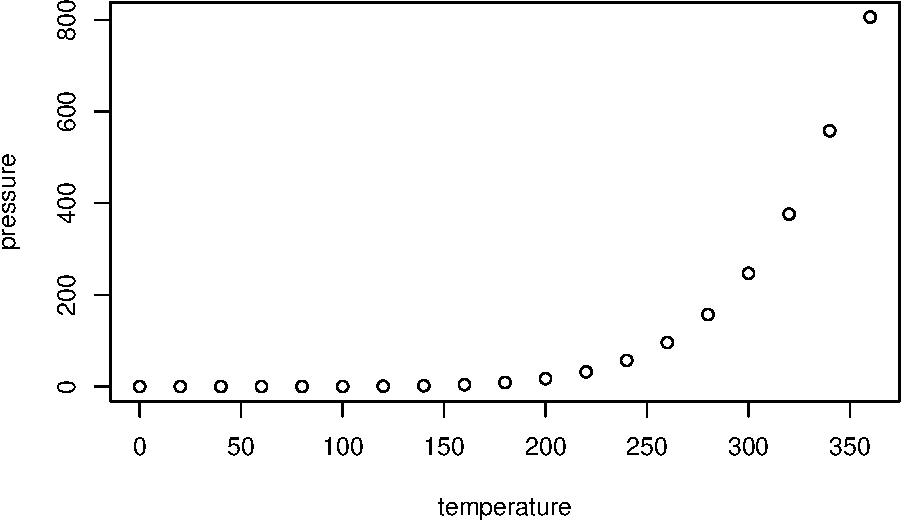
\includegraphics{tesis_files/figure-latex/pressure-1} \end{center}
  
  Note that the \texttt{echo\ =\ FALSE} parameter was added to the code
  chunk to prevent printing of the \textbf{R} code that generated the
  plot. There are plenty of other ways to add chunk options. More
  information is available at \url{http://yihui.name/knitr/options/}.
  
  Another useful chunk option is the setting of \texttt{cache\ =\ TRUE} as
  you see here. If document rendering becomes time consuming due to long
  computations or plots that are expensive to generate you can use knitr
  caching to improve performance. Later in this file, you'll see a way to
  reference plots created in \textbf{R} or external figures.
  
  \hypertarget{loading-and-exploring-data}{\section{Loading and exploring
  data}\label{loading-and-exploring-data}}
  
  Included in this template is a file called \texttt{flights.csv}. This
  file includes a subset of the larger dataset of information about all
  flights that departed from Seattle and Portland in 2014. More
  information about this dataset and its \textbf{R} package is available
  at \url{http://github.com/ismayc/pnwflights14}. This subset includes
  only Portland flights and only rows that were complete with no missing
  values. Merges were also done with the \texttt{airports} and
  \texttt{airlines} data sets in the \texttt{pnwflights14} package to get
  more descriptive airport and airline names.
  
  We can load in this data set using the following command:
  
  \begin{Shaded}
  \begin{Highlighting}[]
  \NormalTok{flights <-}\StringTok{ }\KeywordTok{read.csv}\NormalTok{(}\StringTok{"data/flights.csv"}\NormalTok{)}
  \end{Highlighting}
  \end{Shaded}
  
  The data is now stored in the data frame called \texttt{flights} in
  \textbf{R}. To get a better feel for the variables included in this
  dataset we can use a variety of functions. Here we can see the
  dimensions (rows by columns) and also the names of the columns.
  
  \begin{Shaded}
  \begin{Highlighting}[]
  \KeywordTok{dim}\NormalTok{(flights)}
  \end{Highlighting}
  \end{Shaded}
  
  \begin{verbatim}
  [1] 52808    16
  \end{verbatim}
  
  \begin{Shaded}
  \begin{Highlighting}[]
  \KeywordTok{names}\NormalTok{(flights)}
  \end{Highlighting}
  \end{Shaded}
  
  \begin{verbatim}
   [1] "month"        "day"          "dep_time"     "dep_delay"   
   [5] "arr_time"     "arr_delay"    "carrier"      "tailnum"     
   [9] "flight"       "dest"         "air_time"     "distance"    
  [13] "hour"         "minute"       "carrier_name" "dest_name"   
  \end{verbatim}
  
  Another good idea is to take a look at the dataset in table form. With
  this dataset having more than 50,000 rows, we won't explicitly show the
  results of the command here. I recommend you enter the command into the
  Console \textbf{\emph{after}} you have run the \textbf{R} chunks above
  to load the data into \textbf{R}.
  
  \begin{Shaded}
  \begin{Highlighting}[]
  \KeywordTok{View}\NormalTok{(flights)}
  \end{Highlighting}
  \end{Shaded}
  
  While not required, it is highly recommended you use the \texttt{dplyr}
  package to manipulate and summarize your data set as needed. It uses a
  syntax that is easy to understand using chaining operations. Below I've
  created a few examples of using \texttt{dplyr} to get information about
  the Portland flights in 2014. You will also see the use of the
  \texttt{ggplot2} package, which produces beautiful, high-quality
  academic visuals.
  
  We begin by checking to ensure that needed packages are installed and
  then we load them into our current working environment:
  
  \begin{Shaded}
  \begin{Highlighting}[]
  \CommentTok{# List of packages required for this analysis}
  \NormalTok{pkg <-}\StringTok{ }\KeywordTok{c}\NormalTok{(}\StringTok{"dplyr"}\NormalTok{, }\StringTok{"ggplot2"}\NormalTok{, }\StringTok{"knitr"}\NormalTok{, }\StringTok{"devtools"}\NormalTok{)}
  \CommentTok{# Check if packages are not installed and assign the}
  \CommentTok{# names of the packages not installed to the variable new.pkg}
  \NormalTok{new.pkg <-}\StringTok{ }\NormalTok{pkg[!(pkg %in%}\StringTok{ }\KeywordTok{installed.packages}\NormalTok{())]}
  \CommentTok{# If there are any packages in the list that aren't installed,}
  \CommentTok{# install them}
  \NormalTok{if (}\KeywordTok{length}\NormalTok{(new.pkg))}
    \KeywordTok{install.packages}\NormalTok{(new.pkg, }\DataTypeTok{repos =} \StringTok{"http://cran.rstudio.com"}\NormalTok{)}
  \CommentTok{# Load packages}
  \KeywordTok{library}\NormalTok{(dplyr)}
  \KeywordTok{library}\NormalTok{(ggplot2)}
  \KeywordTok{library}\NormalTok{(knitr)}
  \end{Highlighting}
  \end{Shaded}
  
  The example we show here does the following:
  
  \begin{itemize}
  \item
    Selects only the \texttt{carrier\_name} and \texttt{arr\_delay} from
    the \texttt{flights} dataset and then assigns this subset to a new
    variable called \texttt{flights2}.
  \item
    Using \texttt{flights2}, we determine the largest arrival delay for
    each of the carriers.
  \end{itemize}
  
  \begin{Shaded}
  \begin{Highlighting}[]
  \NormalTok{flights2 <-}\StringTok{ }\NormalTok{flights %>%}\StringTok{ }\NormalTok{dplyr::}\KeywordTok{select}\NormalTok{(carrier_name, arr_delay)}
  \NormalTok{max_delays <-}\StringTok{ }\NormalTok{flights2 %>%}\StringTok{ }\KeywordTok{group_by}\NormalTok{(carrier_name) %>%}
  \StringTok{  }\KeywordTok{summarize}\NormalTok{(}\DataTypeTok{max_arr_delay =} \KeywordTok{max}\NormalTok{(arr_delay, }\DataTypeTok{na.rm =} \OtherTok{TRUE}\NormalTok{))}
  \end{Highlighting}
  \end{Shaded}
  
  We next introduce a useful function in the \texttt{knitr} package for
  making nice tables in \emph{R Markdown} called \texttt{kable}. It
  produces the \LaTeX~code required to make the table and is much easier
  to use than manually entering values into a table by copying and pasting
  values into Excel or \LaTeX. This again goes to show how nice
  reproducible documents can be! There is no need to copy-and-paste values
  to create a table. (Note the use of \texttt{results\ =\ "asis"} here
  which will produce the table instead of the code to create the table.
  You'll learn more about the
  \texttt{\textbackslash{}\textbackslash{}label} later.) The
  \texttt{caption.short} argument is used to include a shorter version of
  the title to appear in the List of Tables at the beginning of the
  document.
  
  \begin{Shaded}
  \begin{Highlighting}[]
  \KeywordTok{kable}\NormalTok{(max_delays, }\DataTypeTok{col.names =} \KeywordTok{c}\NormalTok{(}\StringTok{"Airline"}\NormalTok{, }\StringTok{"Max Arrival Delay"}\NormalTok{),}
        \DataTypeTok{caption =} \StringTok{"Maximum Delays by Airline }\CharTok{\textbackslash{}\textbackslash{}}\StringTok{label\{tab:max_delay\}"}\NormalTok{,}
        \DataTypeTok{caption.short =} \StringTok{"Max Delays by Airline"}\NormalTok{)}
  \end{Highlighting}
  \end{Shaded}
  
  \begin{longtable}[c]{@{}lr@{}}
  \caption{Maximum Delays by Airline \label{tab:max_delay}}\tabularnewline
  \toprule
  Airline & Max Arrival Delay\tabularnewline
  \midrule
  \endfirsthead
  \toprule
  Airline & Max Arrival Delay\tabularnewline
  \midrule
  \endhead
  Alaska Airlines Inc. & 338\tabularnewline
  American Airlines Inc. & 1539\tabularnewline
  Delta Air Lines Inc. & 651\tabularnewline
  Frontier Airlines Inc. & 575\tabularnewline
  Hawaiian Airlines Inc. & 407\tabularnewline
  JetBlue Airways & 273\tabularnewline
  SkyWest Airlines Inc. & 421\tabularnewline
  Southwest Airlines Co. & 694\tabularnewline
  United Air Lines Inc. & 472\tabularnewline
  US Airways Inc. & 347\tabularnewline
  Virgin America & 366\tabularnewline
  \bottomrule
  \end{longtable}
  
  We can further look into the properties of the largest value here for
  American Airlines Inc. To do so, we can isolate the row corresponding to
  the arrival delay of 1539 minutes for American in our original
  \texttt{flights} dataset.
  
  \begin{Shaded}
  \begin{Highlighting}[]
  \NormalTok{flights %>%}\StringTok{ }\NormalTok{dplyr::}\KeywordTok{filter}\NormalTok{(arr_delay ==}\StringTok{ }\DecValTok{1539}\NormalTok{, }
                     \NormalTok{carrier_name ==}\StringTok{ "American Airlines Inc."}\NormalTok{) %>%}
  \StringTok{  }\NormalTok{dplyr::}\KeywordTok{select}\NormalTok{(-}\KeywordTok{c}\NormalTok{(month, day, carrier, dest_name, hour, }
              \NormalTok{minute, carrier_name, arr_delay))}
  \end{Highlighting}
  \end{Shaded}
  
  \begin{verbatim}
    dep_time dep_delay arr_time tailnum flight dest air_time distance
  1     1403      1553     1934  N595AA   1568  DFW      182     1616
  \end{verbatim}
  
  We see that the flight occurred on March 3rd and departed a little after
  2 PM on its way to Dallas/Fort Worth. Lastly, we show how we can
  visualize the arrival delay of all departing flights from Portland on
  March 3rd against time of departure.
  
  \begin{Shaded}
  \begin{Highlighting}[]
  \NormalTok{flights %>%}\StringTok{ }\NormalTok{dplyr::}\KeywordTok{filter}\NormalTok{(month ==}\StringTok{ }\DecValTok{3}\NormalTok{, day ==}\StringTok{ }\DecValTok{3}\NormalTok{) %>%}
  \StringTok{  }\KeywordTok{ggplot}\NormalTok{(}\KeywordTok{aes}\NormalTok{(}\DataTypeTok{x =} \NormalTok{dep_time, }\DataTypeTok{y =} \NormalTok{arr_delay)) +}
  \StringTok{  }\KeywordTok{geom_point}\NormalTok{()}
  \end{Highlighting}
  \end{Shaded}
  
  \begin{center}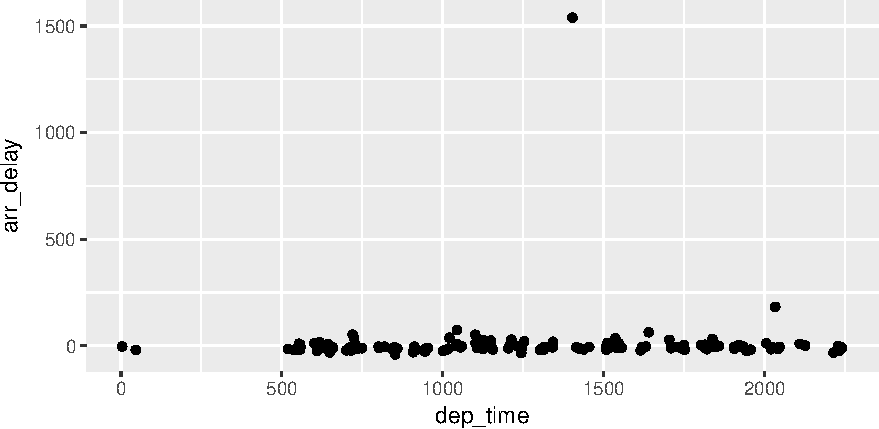
\includegraphics{tesis_files/figure-latex/march3plot-1} \end{center}
  
  \section{Additional resources}\label{additional-resources}
  
  \begin{itemize}
  \item
    \emph{Markdown} Cheatsheet -
    \url{https://github.com/adam-p/markdown-here/wiki/Markdown-Cheatsheet}
  \item
    \emph{R Markdown} Reference Guide -
    \url{https://www.rstudio.com/wp-content/uploads/2015/03/rmarkdown-reference.pdf}
  \item
    Introduction to \texttt{dplyr} -
    \url{https://cran.rstudio.com/web/packages/dplyr/vignettes/introduction.html}
  \item
    \texttt{ggplot2} Documentation -
    \url{http://docs.ggplot2.org/current/}
  \end{itemize}
  
  \chapter{PriA Family}\label{math-sci}
  
  \begin{itemize}
  \tightlist
  \item
    Julian simulation
  \item
    Who has TrpF
  \end{itemize}
  
  \hypertarget{math}{\section{Math}\label{math}}
  
  \TeX~is the best way to typeset mathematics. Donald Knuth designed
  \TeX~when he got frustrated at how long it was taking the typesetters to
  finish his book, which contained a lot of mathematics. One nice feature
  of \emph{R Markdown} is its ability to read \LaTeX~code directly.
  
  If you are doing a thesis that will involve lots of math, you will want
  to read the following section which has been commented out. If you're
  not going to use math, skip over or delete this next commented section.
  
  \section{Chemistry 101: Symbols}\label{chemistry-101-symbols}
  
  Chemical formulas will look best if they are not italicized. Get around
  math mode's automatic italicizing in \LaTeX~by using the argument
  \texttt{\$\textbackslash{}mathrm\{formula\ here\}\$}, with your formula
  inside the curly brackets. (Notice the use of the backticks here which
  enclose text that acts as code.)
  
  So, \(\mathrm{Fe_2^{2+}Cr_2O_4}\) is written
  \texttt{\$\textbackslash{}mathrm\{Fe\_2\^{}\{2+\}Cr\_2O\_4\}\$}.
  
  \noindent Exponent or Superscript: \(\mathrm{O^-}\)
  
  \noindent Subscript: \(\mathrm{CH_4}\)
  
  To stack numbers or letters as in \(\mathrm{Fe_2^{2+}}\), the subscript
  is defined first, and then the superscript is defined.
  
  \noindent Angstrom: \({\AA}\)
  
  \noindent Bullet: CuCl \(\bullet\) \(\mathrm{7H_{2}O}\)
  
  \noindent Double Dagger: \(\ddag\)
  
  \noindent Delta: \(\Delta\)
  
  \noindent Reaction Arrows: \(\longrightarrow\) or
  \(\xrightarrow{solution}\)
  
  \noindent Resonance Arrows: \(\leftrightarrow\)
  
  \noindent Reversible Reaction Arrows: \(\rightleftharpoons\) or
  \(\xrightleftharpoons[ ]{solution}\) (the latter requires the
  \texttt{chemarr} \LaTeX~package which is automatically loaded in this
  template)
  
  \subsection{Typesetting reactions}\label{typesetting-reactions}
  
  You may wish to put your reaction in a figure environment, which means
  that \LaTeX~will place the reaction where it fits and you can have a
  figure caption. You'll see further description of this \textbf{R}
  \texttt{label} function in \protect\hyperlink{refux5flabels}{}. (Note
  the use of the double backslash here as well as the
  \texttt{echo\ =\ FALSE} which hides the code from the output.)
  
  \begin{figure}[h!tbp]
  \begin{center}
  $\mathrm{C_6H_{12}O_6  + 6O_2} \longrightarrow \mathrm{6CO_2 + 6H_2O}$
  \caption{Combustion of glucose}
  \label{fig:comb-gluc}
  \end{center}
  \end{figure}
  
  \subsection{Other examples of
  reactions}\label{other-examples-of-reactions}
  
  \(\mathrm{NH_4Cl_{(s)}}\) \(\rightleftharpoons\)
  \(\mathrm{NH_{3(g)}+HCl_{(g)}}\)
  
  \noindent \(\mathrm{MeCH_2Br + Mg}\) \(\xrightarrow[below]{above}\)
  \(\mathrm{MeCH_2\bullet Mg \bullet Br}\)
  
  \section{Physics}\label{physics}
  
  Many of the symbols you will need can be found on the math page
  \url{http://web.reed.edu/cis/help/latex/math.html} and the Comprehensive
  \LaTeX~Symbol Guide
  (\url{http://mirror.utexas.edu/ctan/info/symbols/comprehensive/symbols-letter.pdf}).
  
  \section{Biology}\label{biology}
  
  You will probably find the resources at
  \url{http://www.lecb.ncifcrf.gov/~toms/latex.html} helpful, particularly
  the links to bsts for various journals. You may also be interested in
  TeXShade for nucleotide typesetting
  (\url{http://homepages.uni-tuebingen.de/beitz/txe.html}). Be sure to
  read the proceeding chapter on graphics and tables.
  
  \hypertarget{refux5flabels}{\chapter{Tables, Graphics, References, and
  Labels}\label{refux5flabels}}
  
  \section{Tables}\label{tables}
  
  In addition to the tables that can be automatically generated from a
  data frame in \textbf{R} that you saw in {[}R Markdown Basics{]} using
  the \texttt{kable} function, you can also create tables using
  \emph{pandoc}. (More information is available at
  \url{http://pandoc.org/README.html\#tables}.) This might be useful if
  you don't have values specifically stored in \textbf{R}, but you'd like
  to display them in table form. Below is an example. Pay careful
  attention to the alignment in the table and hyphens to create the rows
  and columns.
  
  \begin{longtable}[c]{@{}ccc@{}}
  \caption{Correlation of Inheritance Factors for Parents and Child
  \label{tab:inher}}\tabularnewline
  \toprule
  \begin{minipage}[b]{0.29\columnwidth}\centering\strut
  Factors
  \strut\end{minipage} &
  \begin{minipage}[b]{0.47\columnwidth}\centering\strut
  Correlation between Parents \& Child
  \strut\end{minipage} &
  \begin{minipage}[b]{0.16\columnwidth}\centering\strut
  Inherited
  \strut\end{minipage}\tabularnewline
  \midrule
  \endfirsthead
  \toprule
  \begin{minipage}[b]{0.29\columnwidth}\centering\strut
  Factors
  \strut\end{minipage} &
  \begin{minipage}[b]{0.47\columnwidth}\centering\strut
  Correlation between Parents \& Child
  \strut\end{minipage} &
  \begin{minipage}[b]{0.16\columnwidth}\centering\strut
  Inherited
  \strut\end{minipage}\tabularnewline
  \midrule
  \endhead
  \begin{minipage}[t]{0.29\columnwidth}\centering\strut
  Education
  \strut\end{minipage} &
  \begin{minipage}[t]{0.47\columnwidth}\centering\strut
  -0.49
  \strut\end{minipage} &
  \begin{minipage}[t]{0.16\columnwidth}\centering\strut
  Yes
  \strut\end{minipage}\tabularnewline
  \begin{minipage}[t]{0.29\columnwidth}\centering\strut
  Socio-Economic Status
  \strut\end{minipage} &
  \begin{minipage}[t]{0.47\columnwidth}\centering\strut
  0.28
  \strut\end{minipage} &
  \begin{minipage}[t]{0.16\columnwidth}\centering\strut
  Slight
  \strut\end{minipage}\tabularnewline
  \begin{minipage}[t]{0.29\columnwidth}\centering\strut
  Income
  \strut\end{minipage} &
  \begin{minipage}[t]{0.47\columnwidth}\centering\strut
  0.08
  \strut\end{minipage} &
  \begin{minipage}[t]{0.16\columnwidth}\centering\strut
  No
  \strut\end{minipage}\tabularnewline
  \begin{minipage}[t]{0.29\columnwidth}\centering\strut
  Family Size
  \strut\end{minipage} &
  \begin{minipage}[t]{0.47\columnwidth}\centering\strut
  0.18
  \strut\end{minipage} &
  \begin{minipage}[t]{0.16\columnwidth}\centering\strut
  Slight
  \strut\end{minipage}\tabularnewline
  \begin{minipage}[t]{0.29\columnwidth}\centering\strut
  Occupational Prestige
  \strut\end{minipage} &
  \begin{minipage}[t]{0.47\columnwidth}\centering\strut
  0.21
  \strut\end{minipage} &
  \begin{minipage}[t]{0.16\columnwidth}\centering\strut
  Slight
  \strut\end{minipage}\tabularnewline
  \bottomrule
  \end{longtable}
  
  We can also create a link to the table by doing the following:
  \autoref{tab:inher}. If you go back to
  \protect\hyperlink{loading-and-exploring-data}{Loading and exploring
  data} and look at the \texttt{kable} function code, you'll see that I
  added in a similar \texttt{\textbackslash{}\textbackslash{}label} to be
  able to reference that table later. (The extra backslash there is a way
  that \emph{Markdown} interfaces with \LaTeX.) We can create a reference
  to the max delays table: \autoref{tab:max_delay}.
  
  The addition of the \texttt{\textbackslash{}label\{\}} option to the end
  of the table caption allows us to then use the \LaTeX~\texttt{autoref}
  function to produce the link. The \texttt{ref} function in \textbf{R}
  allows for tables and figures to be referenced in the document easily
  without having to directly use the \texttt{autoref} function. It will
  automatically add ``Table'' before your number if you add the ``tab:''
  prefix to your label. Note that this reference could appear anywhere
  throughout the document.
  
  \clearpage
  
  \section{Figures}\label{figures}
  
  If your thesis has a lot of figures, \emph{R Markdown} might behave
  better for you than that other word processor. One perk is that it will
  automatically number the figures accordingly in each chapter. You'll
  also be able to create a label for each figure, add a caption, and then
  reference the figure in a way similar to what we saw with tables
  earlier. If you label your figures, you can move the figures around and
  \emph{R Markdown} will automatically adjust the numbering for you. No
  need for you to remember! So that you don't have to get too far into
  \LaTeX~to do this, a couple \textbf{R} functions have been created for
  you to assist. You'll see their use below.
  
  In the \textbf{R} chunk below, we will load in a picture stored as
  \texttt{reed.jpg} in our main directory. We then give it the caption of
  ``Reed logo'', the label of ``reed'', and specify that this is a figure.
  Note again the use of the \texttt{results\ =\ "asis"} specification to
  automatically include and compile the \LaTeX~code.
  
  \begin{Shaded}
  \begin{Highlighting}[]
  \KeywordTok{label}\NormalTok{(}\DataTypeTok{path =} \StringTok{"figure/reed.jpg"}\NormalTok{, }\DataTypeTok{caption =} \StringTok{"Reed logo"}\NormalTok{, }
        \DataTypeTok{label =} \StringTok{"reed"}\NormalTok{, }\DataTypeTok{type =} \StringTok{"figure"}\NormalTok{)}
  \end{Highlighting}
  \end{Shaded}
  
  \begin{figure}[h!tbp]
  \centering
  
\includegraphics[angle = 0,scale = 1]{figure/reed.jpg}
  \caption[Reed logo]{\normalsize{Reed logo}}
  \label{fig:reed}
  \end{figure}
  
  Here is a reference to the Reed logo: \autoref{fig:reed}. Note the use
  of the inline \textbf{R} code here. By default ``figure'' is specified
  as the type. For clarity, we could have also added the \texttt{label}
  and \texttt{type} to the parameter specifications and this would give us
  the same result: \autoref{fig:reed}.
  
  \clearpage 
  
  Below we will investigate how to save the output of an \textbf{R} plot
  and label it in a way similar to that done above. Recall the
  \texttt{flights} dataset from \protect\hyperlink{rmd-basics}{}. (Note
  that we've shown a different way to reference a section or chapter
  here.) We will next explore a bar graph with the mean flight departure
  delays by airline from Portland for 2014. Note also the use of the
  \texttt{scale} parameter which is discussed on the next page.
  
  \begin{Shaded}
  \begin{Highlighting}[]
  \NormalTok{delay_airline <-}\StringTok{ }\NormalTok{flights %>%}\StringTok{ }\KeywordTok{group_by}\NormalTok{(carrier) %>%}
  \StringTok{  }\KeywordTok{summarize}\NormalTok{(}\DataTypeTok{mean_dep_delay =} \KeywordTok{mean}\NormalTok{(dep_delay)) %>%}
  \StringTok{  }\KeywordTok{ggplot}\NormalTok{(}\KeywordTok{aes}\NormalTok{(}\DataTypeTok{x =} \NormalTok{carrier, }\DataTypeTok{y =} \NormalTok{mean_dep_delay)) +}
  \StringTok{  }\KeywordTok{geom_bar}\NormalTok{(}\DataTypeTok{position =} \StringTok{"identity"}\NormalTok{, }\DataTypeTok{stat =} \StringTok{"identity"}\NormalTok{, }\DataTypeTok{fill =} \StringTok{"red"}\NormalTok{)}
  \KeywordTok{ggsave}\NormalTok{(}\StringTok{"figure/delays.pdf"}\NormalTok{, }\DataTypeTok{plot =} \NormalTok{delay_airline,}
    \DataTypeTok{height =} \DecValTok{3}\NormalTok{, }\DataTypeTok{width =} \DecValTok{6}\NormalTok{)}
  \end{Highlighting}
  \end{Shaded}
  
  \begin{Shaded}
  \begin{Highlighting}[]
  \KeywordTok{label}\NormalTok{(}\DataTypeTok{path =} \StringTok{"figure/delays.pdf"}\NormalTok{, }
        \DataTypeTok{caption =} \StringTok{"Mean Delays by Airline"}\NormalTok{, }
        \DataTypeTok{label =} \StringTok{"delays"}\NormalTok{, }\DataTypeTok{type =} \StringTok{"figure"}\NormalTok{)}
  \end{Highlighting}
  \end{Shaded}
  
  \begin{figure}[h!tbp]
  \centering
  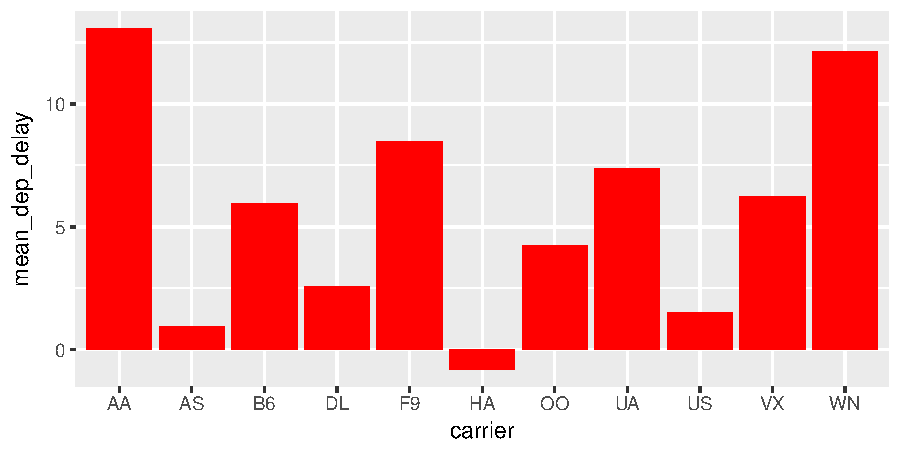
\includegraphics[angle = 0,scale = 1]{figure/delays.pdf}
  \caption[Mean Delays by Airline]{\normalsize{Mean Delays by Airline}}
  \label{fig:delays}
  \end{figure}
  
  A table linking these carrier codes to airline names is available at
  \url{https://github.com/ismayc/pnwflights14/blob/master/data/airlines.csv}.
  
  \clearpage
  
  Next, we will explore the use of the \texttt{scale} parameter which can
  be used to shrink or expand an image. Here we use the mathematical graph
  stored in the ``subdivision.pdf'' file. Note that we didn't specify the
  \texttt{caption\ =} or \texttt{label\ =} here, but we could have.
  
  \begin{Shaded}
  \begin{Highlighting}[]
  \KeywordTok{label}\NormalTok{(}\StringTok{"figure/subdivision.pdf"}\NormalTok{, }\StringTok{"Subdiv. graph"}\NormalTok{, }\StringTok{"subd"}\NormalTok{, }
        \DataTypeTok{scale =} \FloatTok{0.75}\NormalTok{)}
  \end{Highlighting}
  \end{Shaded}
  
  \begin{figure}[h!tbp]
  \centering
  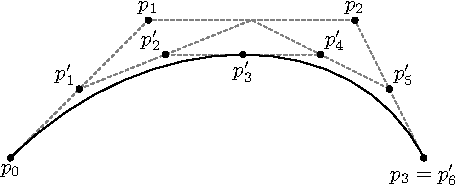
\includegraphics[angle = 0,scale = 0.75]{figure/subdivision.pdf}
  \caption[Subdiv. graph]{\normalsize{Subdiv. graph}}
  \label{fig:subd}
  \end{figure}
  
  Here is a reference to this image: \autoref{fig:subd}. (Move this around
  throughout the document as you wish.)
  
  \subsubsection{More Figure Stuff}\label{more-figure-stuff}
  
  Lastly, we will explore how to rotate figures using the \texttt{angle}
  parameter.
  
  \begin{Shaded}
  \begin{Highlighting}[]
  \KeywordTok{label}\NormalTok{(}\StringTok{"figure/subdivision.pdf"}\NormalTok{, }
        \StringTok{"A Larger Figure, Flipped Upside Down"}\NormalTok{, }
        \DataTypeTok{scale =} \FloatTok{1.5}\NormalTok{,}
        \DataTypeTok{angle =} \DecValTok{180}\NormalTok{,}
        \DataTypeTok{label =} \StringTok{"subd2"}\NormalTok{)}
  \end{Highlighting}
  \end{Shaded}
  
  \begin{figure}[h!tbp]
  \centering
  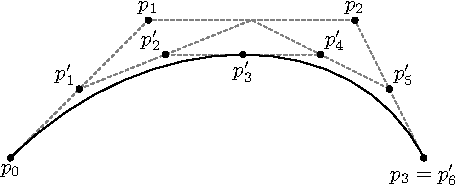
\includegraphics[angle = 180,scale = 1.5]{figure/subdivision.pdf}
  \caption[A Larger Figure, Flipped Upside Down]{\normalsize{A Larger Figure, Flipped Upside Down}}
  \label{fig:subd2}
  \end{figure}
  
  As another example, here is a reference to this figure:
  \autoref{fig:subd2}.
  
  \subsubsection{Common Modifications}\label{common-modifications}
  
  The following figure features the more popular changes thesis students
  want to make to their figures. We can add math to the caption that
  displays below the picture, specify the size of our caption to display
  below the figure (list of sizes available at this
  \href{http://www.emerson.emory.edu/services/latex/latex_169.html\#SEC169}{link}),
  and also specify that a different caption \texttt{alt.cap} be what
  appears in the Table of Figures for this figure.
  
  If you'd like to make further tweaks to figures, you might need to
  invoke some \LaTeX~code. Please email us at
  \href{mailto:data@reed.edu}{\nolinkurl{data@reed.edu}} if you need
  assistance.
  
  \begin{Shaded}
  \begin{Highlighting}[]
  \KeywordTok{label}\NormalTok{(}\StringTok{"figure/subdivision.pdf"}\NormalTok{, }
        \DataTypeTok{caption =} \StringTok{"Subdivision of arc segments"}\NormalTok{,}
        \DataTypeTok{alt.cap =} \StringTok{"You can see that $p_3 = p_6^}\CharTok{\textbackslash{}\textbackslash{}}\StringTok{prime$"}\NormalTok{,}
        \DataTypeTok{cap.size =} \StringTok{"footnotesize"}\NormalTok{,}
        \DataTypeTok{label =} \StringTok{"subd3"}\NormalTok{)}
  \end{Highlighting}
  \end{Shaded}
  
  \begin{figure}[h!tbp]
  \centering
  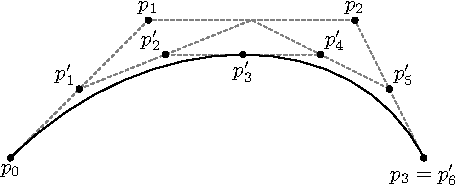
\includegraphics[angle = 0,scale = 1]{figure/subdivision.pdf}
  \caption[Subdivision of arc segments]{\footnotesize{You can see that $p_3 = p_6^\prime$}}
  \label{fig:subd3}
  \end{figure}
  
  \section{Footnotes and Endnotes}\label{footnotes-and-endnotes}
  
  You might want to footnote something.\footnote{footnote text} The
  footnote will be in a smaller font and placed appropriately. Endnotes
  work in much the same way. More information can be found about both on
  the CUS site or feel free to reach out to
  \href{mailto:data@reed.edu}{\nolinkurl{data@reed.edu}}.
  
  \section{Bibliographies}\label{bibliographies}
  
  Of course you will need to cite things, and you will probably accumulate
  an armful of sources. There are a variety of tools available for
  creating a bibliography database (stored with the .bib extension). In
  addition to BibTeX suggested below, you may want to consider using the
  free and easy-to-use tool called Zotero. The Reed librarians have
  created Zotero documentation at
  \url{http://libguides.reed.edu/citation/zotero}. In addition, a tutorial
  is available from Middlebury College at
  \url{http://sites.middlebury.edu/zoteromiddlebury/}.
  
  \emph{R Markdown} uses \emph{pandoc} (\url{http://pandoc.org/}) to build
  its bibliographies. One nice caveat of this is that you won't have to do
  a second compile to load in references as standard \LaTeX~requires. To
  cite references in your thesis (after creating your bibliography
  database), place the reference name inside square brackets and precede
  it by the ``at'' symbol. For example, here's a reference to a book about
  worrying: (Molina \& Borkovec, 1994). This \texttt{Molina1994} entry
  appears in a file called \texttt{thesis.bib} in the \texttt{bib} folder.
  This bibliography database file was created by a program called BibTeX.
  You can call this file something else if you like (look at the YAML
  header in the main .Rmd file) and, by default, is to placed in the
  \texttt{bib} folder.
  
  For more information about BibTeX and bibliographies, see our CUS site
  (\url{http://web.reed.edu/cis/help/latex/index.html})\footnote{Reed~College
    (2007)}. There are three pages on this topic: \emph{bibtex} (which
  talks about using BibTeX, at
  \url{http://web.reed.edu/cis/help/latex/bibtex.html}),
  \emph{bibtexstyles} (about how to find and use the bibliography style
  that best suits your needs, at
  \url{http://web.reed.edu/cis/help/latex/bibtexstyles.html}) and
  \emph{bibman} (which covers how to make and maintain a bibliography by
  hand, without BibTeX, at
  \url{http://web.reed.edu/cis/help/latex/bibman.html}). The last page
  will not be useful unless you have only a few sources.
  
  If you look at the YAML header at the top of the main .Rmd file you can
  see that we can specify the style of the bibliography by referencing the
  appropriate csl file. You can download a variety of different style
  files at \url{https://www.zotero.org/styles}. Make sure to download the
  file into the csl folder.
  
  \paragraph{Tips for Bibliographies}\label{tips-for-bibliographies}
  
  \begin{itemize}
  \tightlist
  \item
    Like with thesis formatting, the sooner you start compiling your
    bibliography for something as large as thesis, the better. Typing in
    source after source is mind-numbing enough; do you really want to do
    it for hours on end in late April? Think of it as procrastination.
  \item
    The cite key (a citation's label) needs to be unique from the other
    entries.
  \item
    When you have more than one author or editor, you need to separate
    each author's name by the word ``and'' e.g.
    \texttt{Author\ =\ \{Noble,\ Sam\ and\ Youngberg,\ Jessica\},}.
  \item
    Bibliographies made using BibTeX (whether manually or using a manager)
    accept \LaTeX~markup, so you can italicize and add symbols as
    necessary.
  \item
    To force capitalization in an article title or where all lowercase is
    generally used, bracket the capital letter in curly braces.
  \item
    You can add a Reed Thesis citation\footnote{Noble (2002)} option. The
    best way to do this is to use the phdthesis type of citation, and use
    the optional ``type'' field to enter ``Reed thesis'' or
    ``Undergraduate thesis.''
  \end{itemize}
  
  \section{Anything else?}\label{anything-else}
  
  If you'd like to see examples of other things in this template, please
  contact the Data @ Reed team (email
  \href{mailto:data@reed.edu}{\nolinkurl{data@reed.edu}}) with your
  suggestions. We love to see people using \emph{R Markdown} for their
  theses, and are happy to help.
  
  \chapter*{Conclusion}\label{conclusion}
  \addcontentsline{toc}{chapter}{Conclusion}
  
  \setcounter{chapter}{4} \setcounter{section}{0}
  
  If we don't want Conclusion to have a chapter number next to it, we can
  add the \texttt{\{.unnumbered\}} attribute. This has an unintended
  consequence of the sections being labeled as 3.6 for example though
  instead of 4.1. The \LaTeX~commands immediately following the Conclusion
  declaration get things back on track.
  
  \subsubsection{More info}\label{more-info}
  
  And here's some other random info: the first paragraph after a chapter
  title or section head \emph{shouldn't be} indented, because indents are
  to tell the reader that you're starting a new paragraph. Since that's
  obvious after a chapter or section title, proper typesetting doesn't add
  an indent there.
  
  \appendix
  
  \chapter{The First Appendix}\label{the-first-appendix}
  
  This first appendix includes all of the R chunks of code that were
  hidden throughout the document (using the \texttt{include\ =\ FALSE}
  chunk tag) to help with readibility and/or setup.
  
  \subsubsection{In the main Rmd file:}\label{in-the-main-rmd-file}
  
  \begin{Shaded}
  \begin{Highlighting}[]
  \CommentTok{# This chunk ensures that the reedtemplates package is}
  \CommentTok{# installed and loaded. This reedtemplates package includes}
  \CommentTok{# the template files for the thesis and also two functions}
  \CommentTok{# used for labeling and referencing}
  \NormalTok{if(!}\KeywordTok{require}\NormalTok{(devtools))}
    \KeywordTok{install.packages}\NormalTok{(}\StringTok{"devtools"}\NormalTok{, }\DataTypeTok{repos =} \StringTok{"http://cran.rstudio.com"}\NormalTok{)}
  \NormalTok{if(!}\KeywordTok{require}\NormalTok{(reedtemplates))\{}
    \KeywordTok{library}\NormalTok{(devtools)}
    \NormalTok{devtools::}\KeywordTok{install_github}\NormalTok{(}\StringTok{"ismayc/reedtemplates"}\NormalTok{)}
  \NormalTok{\}}
  \KeywordTok{library}\NormalTok{(reedtemplates)}
  \end{Highlighting}
  \end{Shaded}
  
  \subsubsection{\texorpdfstring{In
  \protect\hyperlink{refux5flabels}{}:}{In :}}\label{in}
  
  \begin{Shaded}
  \begin{Highlighting}[]
  \CommentTok{# This chunk ensures that the reedtemplates package is}
  \CommentTok{# installed and loaded. This reedtemplates package includes}
  \CommentTok{# the template files for the thesis and also two functions}
  \CommentTok{# used for labeling and referencing}
  \NormalTok{if(!}\KeywordTok{require}\NormalTok{(devtools))}
    \KeywordTok{install.packages}\NormalTok{(}\StringTok{"devtools"}\NormalTok{, }\DataTypeTok{repos =} \StringTok{"http://cran.rstudio.com"}\NormalTok{)}
  \NormalTok{if(!}\KeywordTok{require}\NormalTok{(dplyr))}
      \KeywordTok{install.packages}\NormalTok{(}\StringTok{"dplyr"}\NormalTok{, }\DataTypeTok{repos =} \StringTok{"http://cran.rstudio.com"}\NormalTok{)}
  \NormalTok{if(!}\KeywordTok{require}\NormalTok{(ggplot2))}
      \KeywordTok{install.packages}\NormalTok{(}\StringTok{"ggplot2"}\NormalTok{, }\DataTypeTok{repos =} \StringTok{"http://cran.rstudio.com"}\NormalTok{)}
  \NormalTok{if(!}\KeywordTok{require}\NormalTok{(reedtemplates))\{}
    \KeywordTok{library}\NormalTok{(devtools)}
    \NormalTok{devtools::}\KeywordTok{install_github}\NormalTok{(}\StringTok{"ismayc/reedtemplates"}\NormalTok{)}
    \NormalTok{\}}
  \KeywordTok{library}\NormalTok{(reedtemplates)}
  \NormalTok{flights <-}\StringTok{ }\KeywordTok{read.csv}\NormalTok{(}\StringTok{"data/flights.csv"}\NormalTok{)}
  \end{Highlighting}
  \end{Shaded}
  
  \chapter{The Second Appendix, for
  Fun}\label{the-second-appendix-for-fun}
  
  \backmatter
  
  \chapter{References}\label{references}
  
  \noindent
  
  \setlength{\parindent}{-0.20in} \setlength{\leftskip}{0.20in}
  \setlength{\parskip}{8pt}
  
  \hypertarget{refs}{}
  \hypertarget{ref-angel2000}{}
  Angel, E. (2000). \emph{Interactive computer graphics : A top-down
  approach with openGL}. Boston, MA: Addison Wesley Longman.
  
  \hypertarget{ref-angel2001}{}
  Angel, E. (2001a). \emph{Batch-file computer graphics : A bottom-up
  approach with quickTime}. Boston, MA: Wesley Addison Longman.
  
  \hypertarget{ref-angel2002a}{}
  Angel, E. (2001b). \emph{Test second book by angel}. Boston, MA: Wesley
  Addison Longman.
  
  \hypertarget{ref-Molina1994}{}
  Molina, S. T., \& Borkovec, T. D. (1994). The Penn State worry
  questionnaire: Psychometric properties and associated characteristics.
  In G. C. L. Davey \& F. Tallis (Eds.), \emph{Worrying: Perspectives on
  theory, assessment and treatment} (pp. 265--283). New York: Wiley.
  
  \hypertarget{ref-noble2002}{}
  Noble, S. G. (2002). \emph{Turning images into simple line-art}
  (Undergraduate thesis). Reed College.
  
  \hypertarget{ref-reedweb2007}{}
  Reed~College. (2007, March). LaTeX your document. Retrieved from
  \url{http://web.reed.edu/cis/help/LaTeX/index.html}


  % Index?

\end{document}

